\begin{frame}{Texture}{Définition}
\begin{block}{Définition}

\textit{Région spatiale d'une image présentant une organisation une organisation spatiale homogène des niveaux de luminance}.

Structure en deux dimensions :

\begin{itemize}
    \item Première dimension :  primitives formant la texture ;
    \item Seconde dimension : organisation spatiale de ces primitives entre elles.
\end{itemize}

\end{block}

\end{frame}

\begin{frame}{Texture}{Types}
\begin{block}{Types de texture :}

\begin{itemize}
    \item \textbf{Macrotexture} : texture structurée, pour laquelle on peut extraire facilement un motif de base et les lois d'assemblage des primitives entre elles ;
    \item \textbf{Microtexture} : texture aléatoire, avec un aspect désorganisé, mais qui donne une impression visuelle relativement homogène.
\end{itemize}

\end{block}
\end{frame}

\begin{frame}{Texture}{Exemples}

\begin{figure}
   \begin{minipage}[c]{.46\linewidth}
	  \centering
      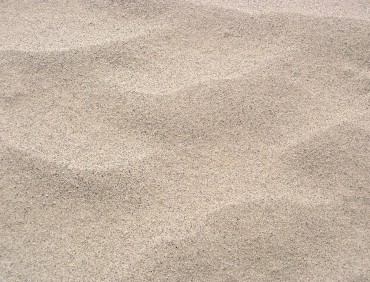
\includegraphics[scale=0.32]{images/sable.jpg}
      \caption{Exemple microtexture}
   \end{minipage} \hfill
   \begin{minipage}[c]{.46\linewidth}
      \centering
      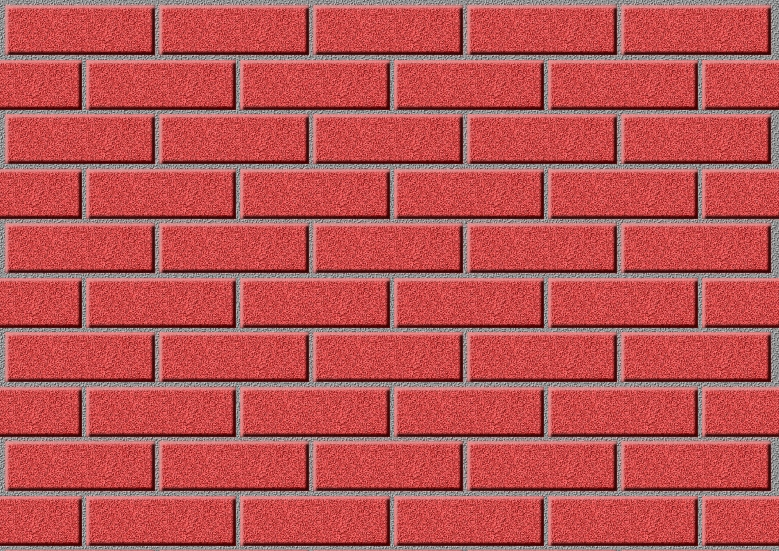
\includegraphics[scale=0.16]{images/briques.jpg}
      \caption{Exemple macrotexture}
   \end{minipage}
\end{figure}

\end{frame}


\begin{frame}{Texture}{Matrice de cooccurrence}

\begin{block}{Principe :}

Méthode statistique basée sur le niveau de gris d'une image (de 1 à 8 au maximum). Cette méthode compte le nombre de paires de pixels similaires dans une image et stocke les résultats dans une matrice de cooccurrence (taille $n \times n$ avec $n$ le niveau de gris maximum).

\end{block}

\end{frame}

\begin{frame}{Texture}{Matrice de cooccurrence}

\begin{exampleblock}{Exemple}

\[
 I = \begin{pmatrix}
     1 & 8 & 1 & 8 \\
     2 & 1 & 1 & 8 \\
     5 & 4 & 3 & 7 \\     
 \end{pmatrix}
, 
 C = \begin{pmatrix}
     1 & 0 & 0 & 0 & 0 & 0 & 0 & 3 \\
     1 & 0 & 0 & 0 & 0 & 0 & 0 & 0 \\
     0 & 0 & 0 & 0 & 0 & 0 & 1 & 0 \\
     0 & 0 & 1 & 0 & 0 & 0 & 0 & 0 \\
     0 & 0 & 0 & 1 & 0 & 0 & 0 & 0 \\
     0 & 0 & 0 & 0 & 0 & 0 & 0 & 0 \\
     0 & 0 & 0 & 0 & 0 & 0 & 0 & 0 \\
     1 & 0 & 0 & 0 & 0 & 0 & 0 & 0 \\   
 \end{pmatrix}
\]

avec $I$ l'image en niveau de gris et $C$ la matrice de cooccurrence.

\end{exampleblock}

\end{frame}

\begin{frame}{Texture}{Conclusion}

\begin{block}{Avantages :}

\begin{itemize}
    \item Simple à mettre en oeuvre ;
    \item Relativement robuste aux mouvements.
\end{itemize}

\end{block}

\begin{block}{Inconvénients :}

\begin{itemize}
    \item Basée sur les niveaux de gris, donc peu robuste aux transitions avec un effet de fondu ;
   	\item Peu robuste aux changement d'intensité d'une couleur ;
   	\item Peu robuste à l'apparition de nouveaux objets sur une scène.
\end{itemize}

\end{block}

\end{frame}

\begin{frame}{Flux optique}{Définition}

\begin{block}{Définition :}

Le flux optique (ou flot optique) représente le mouvement apparent des objets présents sur une image et est basé sur la luminance.

Pour un pixel donné, la relation suivante est vérifiée entre deux images consécutives :

$I(x, y, t) = I(x + \Delta x, y + \Delta y, t + \Delta t)$ avec $I$ la luminosité de l'image.

\end{block}

\end{frame}

\begin{frame}{Flux optique}{Ecriture différentielle}

\begin{block}{Equation du flux optique :}

En supposant que le mouvement petit et constant, on obtient :

\[	
	\begin{array}{c}
	     \frac{dI(x, y, t)}{\Delta t} = 0 \\
	     \frac{dI(x, y, t)}{\Delta t} = \frac{\partial I}{\partial x}.\frac{\Delta x}{\Delta t} + \frac{\partial I}{\partial y}.\frac{\Delta y}{\Delta t} + \frac{\partial I}{\partial t}\\
	\end{array}
\]

Soit :

\[
	I_x.V_x + I_y.V_y = -I_t
\]
avec $V_x$ et $V_y$, le flux optique (ou les composants $(x, y)$ de la vitesse) et $I_x$, $I_y$ et $I_t$ les dérivées partielles de l'intensité de l'image.

\end{block}

\end{frame}

\begin{frame}{Flux optique}{Gradient et filtre de Sobel}

\begin{block}{Principe :}

\begin{itemize}
	\item Définition des matrices de convolution :
	$
		C_1 = \begin{pmatrix}
			1 & 0 & -1 \\
			2 & 0 & -2 \\
			1 & 0 & -1 \\
		\end{pmatrix}
	$
	 et 
	$	
		C_2 = \begin{pmatrix}
			1 & 2 & 1 \\
			0 & 0 & 0 \\
			-1 & -2 & -1 \\
		\end{pmatrix}
	$
	\item Calcul des dérivées partielles ($G_x$ et $G_y$) :
	$
		G_x = C_1 \ast Img
	$
	 et 
	$	
		G_y = C_2 \ast Img
	$
	\item Combinaison des gradients horizontaux et verticaux : $G = \sqrt{G_x^2 + G_y^2}$
\end{itemize}

\end{block}

\end{frame}

\begin{frame}{Flux optique}{Méthode de Lucas-Kanade}

\begin{block}{Principe :}
On suppose que le déplacement d'un pixel $p$ est petit et constant dans son voisinage :
\begin{itemize}
	\item Sélectionner une fenêtre centrée sur le pixel $p$ dont on cherche la vitesse ;
	\item Réécrire l'équation du flux optique comme un système d'équation ;
	\item Résoudre ce système d'équations par la méthode des moindres carrés.
\end{itemize}

\end{block}

\end{frame}

\begin{frame}{Flux optique}{Conclusion}

\begin{block}{Avantages :}

\begin{itemize}
	\item Relativement robuste aux mouvements;
	\item Relativement robuste aux changements d'intensité de couleur.
\end{itemize}

\end{block}

\begin{block}{Inconvénients :}

\begin{itemize}
	\item Peu robuste aux transitions avec un effet de fondu ;
	\item Assez lourd à mettre en place ;
	\item Peu robuste lors de l'arrivé ou de la disparition d'un objet dans la scène.
\end{itemize}

\end{block}

\end{frame}
